\section{Method}
在本节中,我们给出了我们提出的网络结构和参数,以及loss的选择。
\subsection{整体的网络结构}
假设$x\in R^{MN \times{1}}$是已被测量得出的在稀疏下的正弦图,$y\in R^{HWS\times{1}}$是其对应的高质量的CT图像。我们的任务是找到一个函数f,其满足\begin{equation}y = f(x)\end{equation}其中M和N分别表示探测器的数量和投影角度,$H\times{W}\times{S}$表示CT图像Y的分辨率,S是CT图片切片的数量,对于fan beam geometry来说,S的值为1。我们将使用深度学习网络去拟合函数f,网络的整体架构和流程如图1所示。 \par
\begin{figure}
	\centering
	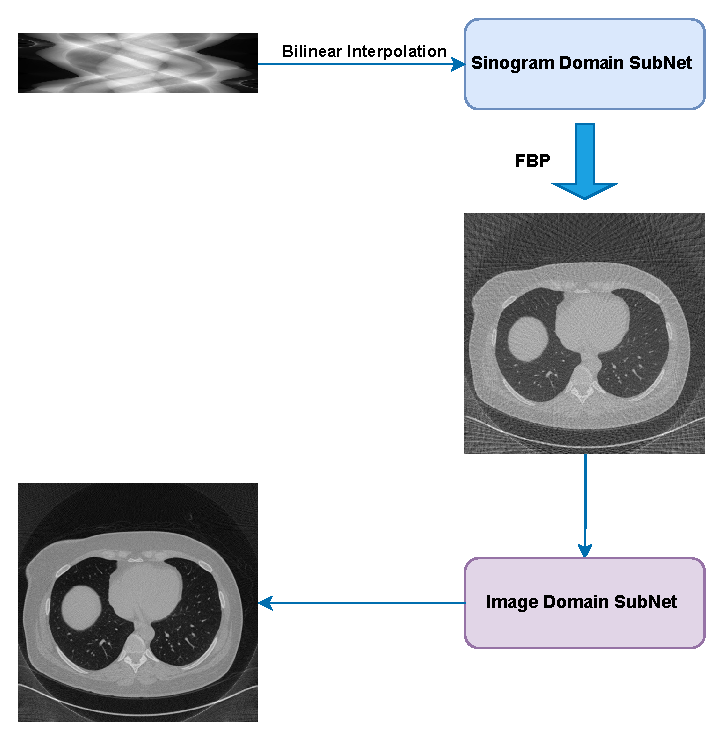
\includegraphics[height=8cm,width=8cm]{1.eps}
	\caption{PLformer的整体架构,该网络有三个阶段:Sinogram Domain SubNet,Filter BackProjection(FBP),和Image Domain SubNet。}
	\label{fig1}
\end{figure}
网络整体由三个阶段组成,首先通过Sinogram Domain SubNet对双线性插值后的稀疏正弦图进行重建,然后通过FBP算法完成投影域到图像域的转换,最后通过Image Domain SubNet重建出高质量的CT图片。
\subsection{Parallel LeWinTransformer Block(PLB)}
过去基于卷积的神经网络的特征提取是非常成功的,但卷积操作需要不断堆积卷积层来完成对图像从局部信息到全局信息的提取,不断堆积的卷积层慢慢地扩大了感受野直至覆盖整个图像。但是transformer并不假定从局部信息开始,而且一开始就可以拿到全局信息,尽管训练难度更大一些(如所需要的数据集要更大些,以及所需要学习的参数量更多),但是一旦完成好训练,更早得到全局信息的优势会使得效果更好。受到Swin Transformer\cite{liu2021Swin}以及Uformer\cite{wang2021uformer}的启发,我们使用由 non-overlapping window-based Multi-head Self-Attention (W-MSA) 和 Locally-enhanced Feed-Forward Network (LeFF) 所组成的 locally-enhanced window (LeWin) Transformer 来获取图像信息,其中W-MSA用来捕获全局信息,而LeFF用来捕获局部信息。LeWin Transformer的计算表示为
:
\begin{equation}\begin{aligned}&X^{'}_{n} = \mathrm{W\mbox{-}MSA}(\mathrm{LN}(X_{n-1}))+X_{n}   \\&X_{n} = \mathrm{LeFF}(\mathrm{LN}(X^{'}_{n}))+X^{'}_{n}\end{aligned}\end{equation}
其中LN表示the layer normalization,$X^{'}_{n}$和$X_{n}$分别为W-MSA和LeFF的输出。\par

由于切Patch会导致边界信息的不易捕获,如图2所示,我们提出Parallel LeWinTransformer Block(PLB),将 transformer block并行concatenate,并且shift互不相等。之后,使用Point-Wise Convolution\cite{2017Xception}将二者互补,达到弥补边界信息的作用。整个过程可表示为:
\begin{equation}\begin{aligned}X_{l} = \mathrm{PW}(\mathrm{Concat}(\mathrm{LeWin_1}(X_{l-1}),\mathrm{LeWin_2}(X_{l-1}))+X_{l-1} \end{aligned}\end{equation}其中Concat表示拼接操作,$\mathrm{LeWin}_i(i=1,2)$分别表示shift=0和shift=n的LeWin Transformer Block。PW表示Point-Wise Convolution。\par GELU\cite{hendrycks2016gelu}作为激活函数。
\begin{figure}
	\centering
	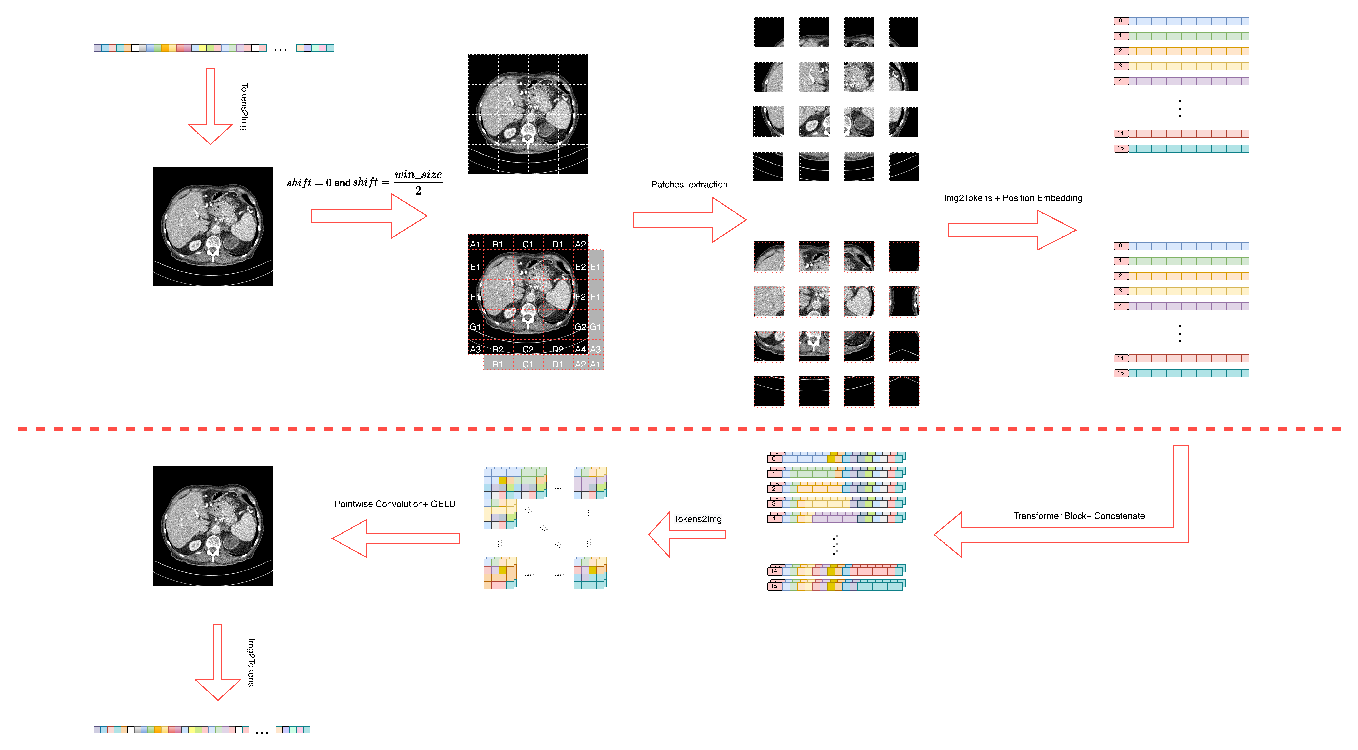
\includegraphics[height=5cm,width=10cm]{5.eps}
	\caption{Parallel LeWinTransformer Block(PLB)整体架构。}
	\label{fig2}
\end{figure}

\subsection{Sinogram Domain SubNet}
如图3 Part1所示,我们使用5块PLB来组成Sinogram Domain SubNet。设经过插值之后的投影图像为$x\in R^{M\times{N}\times{1}}$,首先通过 Input Projection 进行特征提取并Flatten

\subsection{Sinogram Domain SubNet}
如图3 Part1所示,Sinogram Domain SubNet采用编码-解码的架构,他由5部分组成。首先通过Input Projection对输入的Sinogram 2-D图片通过一个3x3的卷积提取特征并通过Flatten将每个特征变成1-D的token。然后在这些token上应用PFLB来获取长范围依赖,并且根据LeWinTransformer可以通过层次化的表示来减少token数量的特点,我们在PFLB之后对采用token长度变为1/4,token维数加倍的下采样,这样token的总数会减半。在两层encoder之后的使用PFLB作为bottleneck layer。我们同样使用2层decoder来进行token重建。和encoder相似,decoder由token长度$\times4$,维数减半的上采样和PFLB组成。但不同的是我们将上采样和对应encoder阶段的token合并起来,并用point-wise convolution进行融合之后在输入到PFLB中。最后通过Output Projection将1-D的token转为2-D的特征,再用一个3x3的卷积获取residual image。假设输入的正旋图为$X$,得到的residual image为$R$。则我们最终的结果定义为$X^{'}=X+R$,而正常采样下的正弦图为$Y$,我们使用 the mean square error (MSE) 作为我们的损失函数:\begin{equation}\begin{aligned}
l(X^{'},Y) = \mid X^{'}-Y\mid^{2}\end{aligned}
\end{equation}\par
\textbf{参数选择}: 我们选择特征的通道数为16,并且在Input Projection和Output Projection的卷积之后使用LeakyReLU leaky rectified linear activation functions (LReLUs)\cite{2013Rectifier} 去稳定我们的训练。下采样我们使用参数为kernel size为4,stride为2,padding为1的卷积,而上采样使用kernel size为2,stride为2的转置卷积。对于每个W-MSA,我们使用了参数为0.5的Dropout\cite{2014Dropout}来防止过拟合。最后,我们将卷积层中的权重初始化为正态分布($\mu$= 0.0,$\sigma$= 0.02)。
\begin{figure}
	\centering
	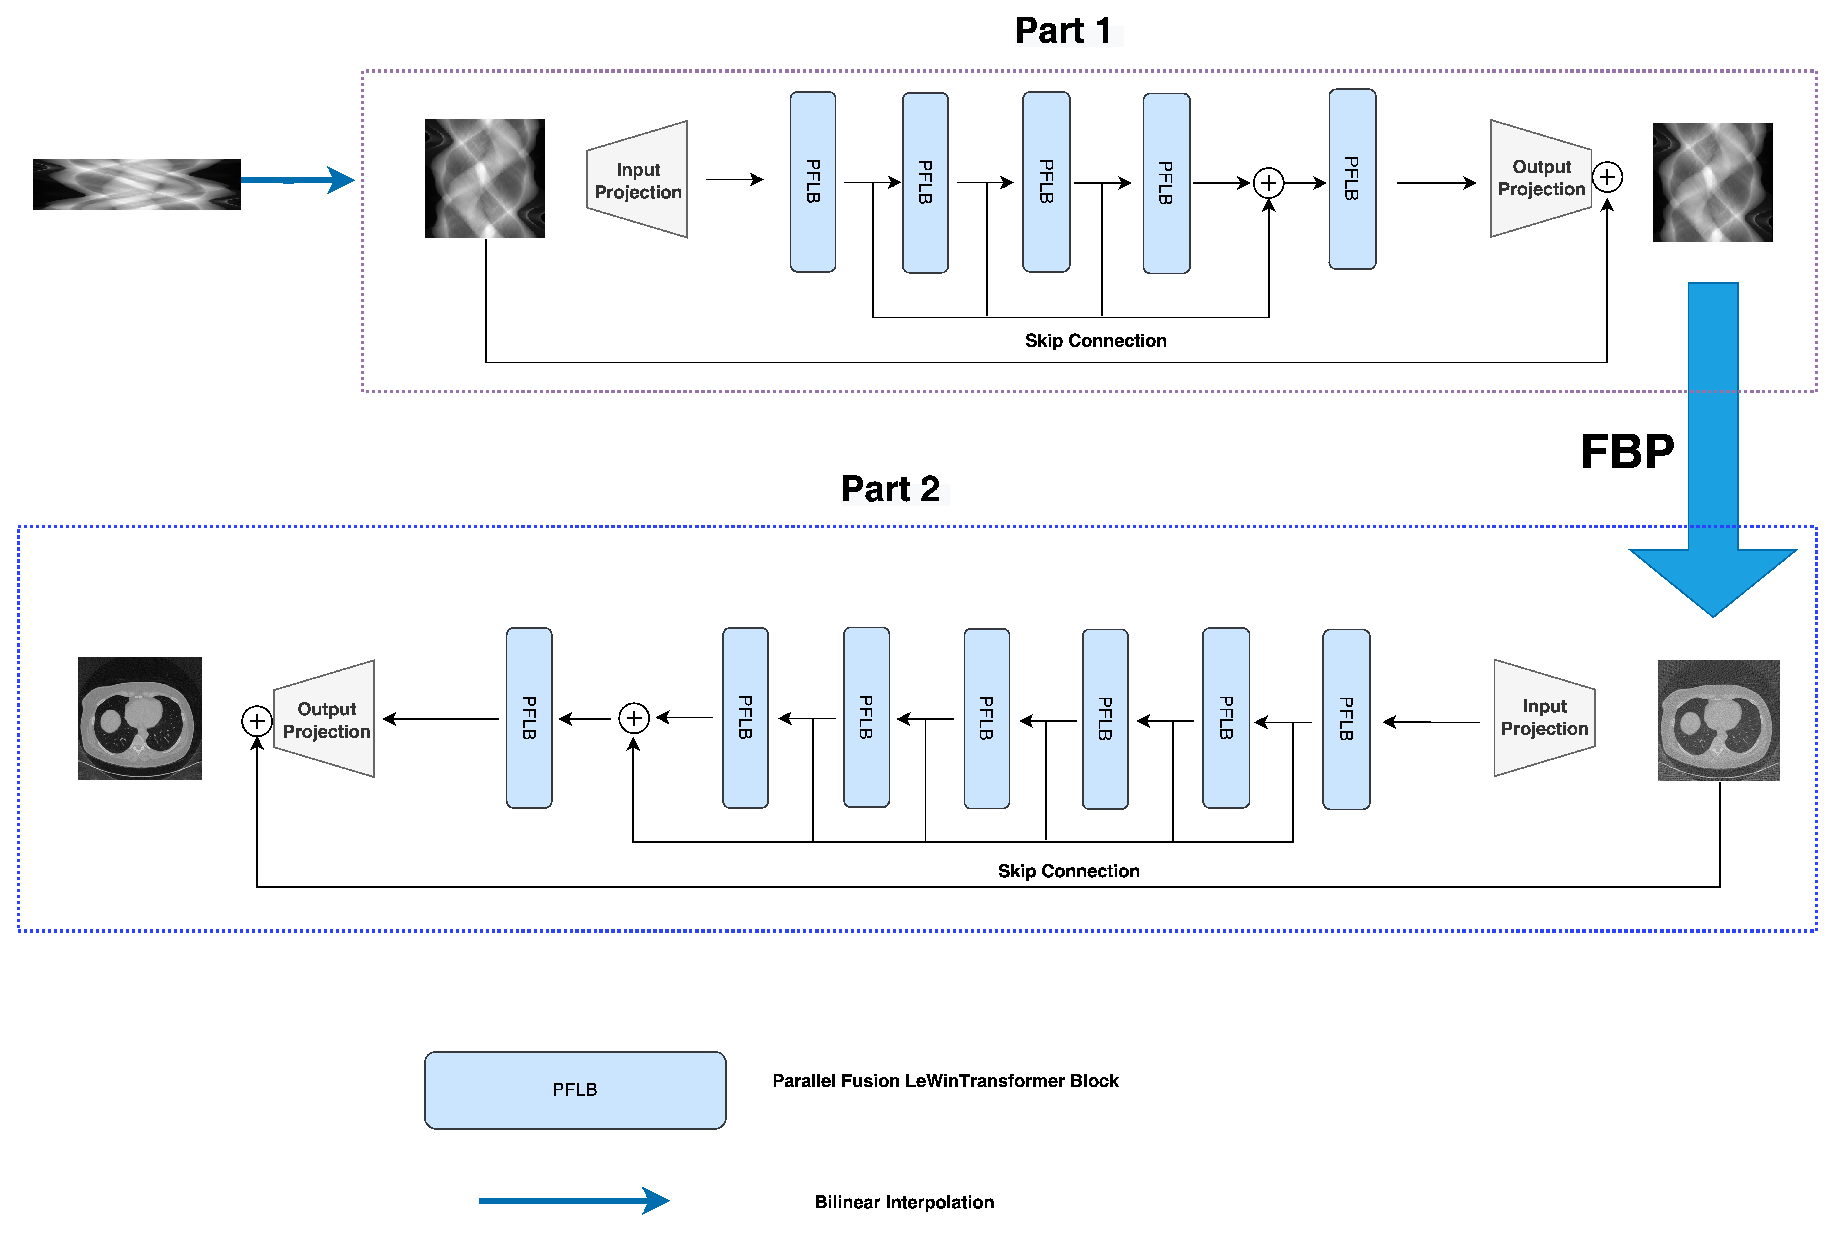
\includegraphics[height=8cm,width=12cm]{6.eps}
	\caption{PLFormer,Part1为Sinogram Domain SubNet,Part2为Image Domain SubNet。}
	\label{fig3}
\end{figure}
\subsection{Image Domain SubNet}
由于FBP重构的CT图像受到条纹伪影和噪声的影响而退化,所以我们通过Image Domain SubNet来重建出高质量的CT图。如图3 Part2所示,Image Domain SubNet整体架构和Sinogram Domain SubNet类似。不同的是为了得到更多的token,我们分别选用了5层的encoder layer和decoder layer,以及将特征的通道数设为18。为了加快模型的收敛速度以及使得模型的performance更好,我们使用了Charbonnier Loss\cite{2017Fast}作为损失函数:
\begin{equation}\begin{aligned}
Charbonnier\_Loss(X^{'},Y) = \sqrt{(X^{'}-Y)^{2} + \epsilon^{2}} \end{aligned}
\end{equation}
其中$X^{'}$表示我们最终重建得到的CT图,$Y$是高质量的CT图,$\epsilon$的值为常量$10^{-3}$。\par